\scanpage{86}
\mspage{39}

\margin{Je ne suis pas \unsure{très sûr|sûr} que l'hypothèse que $J\cap L=\phi$ soit vrai-\
ment essentielle, ou celle que $J\prec L$, \unsure{en fait on} dans ces passages.}

Soient $J$ et $L$ deux bandes \uline{disjointes}, avec $J\prec L$ dans une bande $I'$ telles que $J$ est un idéal de $I'$, $L$ un coidéal de $I'$,
\[
I'\subset\widetilde J\cap\bar L\qquad(\text{en fait on aura alors }I'=\widetilde J\cap\bar L)
\]
Soit $J'=I'\setminus L$, donc dans $I'$ on a une inclusion d'idéaux
\[J\subset J'\subset I'\]
(car $J\cap L=\phi$). Considérons \deleted{$X_J^*\subset X_{J'}^*$} le diagramme

\margin{$\Sigma_{JL}=\dot T_J\cap\Sigma_L$, où
\[
\begin{aligned}
T_J&\overset{\mathrm{def}}{=}\deleted{\unsure{T_J\cap\Sigma_J}}\ ;\ \Sigma_J\cap\bigcup_{j\in J}\unsure{T_j^{\deleted{\circ}}|\dot T_j}\\
\mathring T_J&=\mathring T_{\bar J}\cap\Sigma_J=\Sigma_J\cap\bigcup_{j\in J}\mathring T_j,\\
\dot T_J&=T_J\setminus\mathring T_J,\\
\dot T_J&\overset{?}{=}\underset{\substack{d\in\mathrm{Drap}(I)\\\text{él. initial de }d\text{ est}\in J}}{\lim_{\longrightarrow}}\Sigma_d\quad(=\Sigma_{J,I}),\\
\Sigma_{J,L}&\overset{?}{=}\underset{\substack{\text{él. initial de }d\text{ est}\in J\\\text{--- final \deleted{\unsure{est}}}\in L\\d\in\mathrm{Drap}(J\cup L)}}{\lim_{\longrightarrow}}\Sigma_d
\end{aligned}
\]}

\diagram{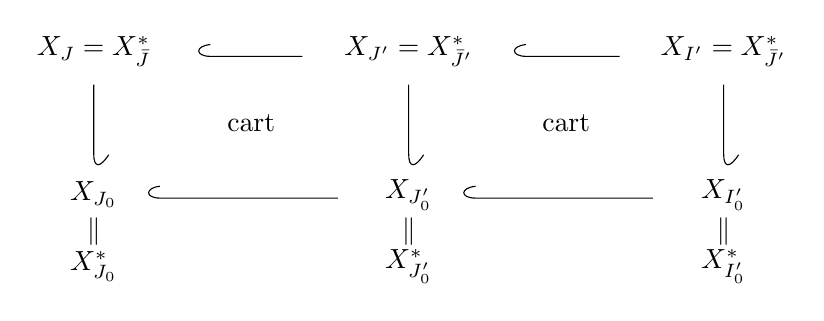
\begin{tikzpicture}[x=1cm,y=1cm]
\node at (0,0) {$X_J=X_{\bar J}^*$};
\node at (4,0) {$X_{J'}=X_{\bar J'}^*$};
\node at (8,0) {$X_{I'}=X_{\bar J'}^*$};
\draw (1.48,0.09) .. controls (1.28,0.07) and (1.29,-0.06) .. (1.48,-0.06) -- (2.65,-0.06);
\draw (5.49,0.09) .. controls (5.29,0.07) and (5.30,-0.06) .. (5.49,-0.06) -- (6.68,-0.06);
\draw (0,-0.42) -- (0,-1.30) .. controls (0,-1.48) and (0.08,-1.48) .. (0.19,-1.31);
\draw (4,-0.42) -- (4,-1.30) .. controls (4,-1.48) and (4.08,-1.48) .. (4.19,-1.31);
\draw (8,-0.42) -- (8,-1.30) .. controls (8,-1.48) and (8.08,-1.48) .. (8.19,-1.31);
\node at (2,-0.90) {cart};
\node at (6,-0.90) {cart};
\node at (0,-1.82) {$X_{J_0}$};
\node at (4,-1.82) {$X_{J'_0}$};
\node at (8,-1.82) {$X_{I'_0}$};
\draw (0.84,-1.71) .. controls (0.65,-1.73) and (0.65,-1.86) .. (0.84,-1.86) -- (3.10,-1.86);
\draw (4.85,-1.71) .. controls (4.65,-1.73) and (4.65,-1.86) .. (4.85,-1.86) -- (7.10,-1.86);
\node at (0,-2.28) {$\Vert$};
\node at (4,-2.28) {$\Vert$};
\node at (8,-2.28) {$\Vert$};
\node at (0,-2.73) {$X_{J_0}^*$};
\node at (4,-2.73) {$X_{J'_0}^*$};
\node at (8,-2.73) {$X_{I'_0}^*$};
\end{tikzpicture}}

correspondant au diagramme
\diagram{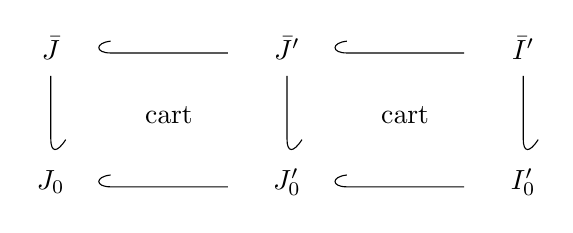
\begin{tikzpicture}[x=1cm,y=1cm]
\node at (0,0) {$\bar J$};
\node at (3,0) {$\bar J'$};
\node at (6,0) {$\bar I'$};
\draw (0.76,0.09) .. controls (0.56,0.07) and (0.56,-0.06) .. (0.76,-0.06) -- (2.25,-0.06);
\draw (3.76,0.09) .. controls (3.56,0.07) and (3.56,-0.06) .. (3.76,-0.06) -- (5.25,-0.06);
\draw (0,-0.35) -- (0,-1.15) .. controls (0,-1.33) and (0.08,-1.33) .. (0.19,-1.16);
\draw (3,-0.35) -- (3,-1.15) .. controls (3,-1.33) and (3.08,-1.33) .. (3.19,-1.16);
\draw (6,-0.35) -- (6,-1.15) .. controls (6,-1.33) and (6.08,-1.33) .. (6.19,-1.16);
\node at (1.5,-0.85) {cart};
\node at (4.5,-0.85) {cart};
\node at (0,-1.70) {$J_0$};
\node at (3,-1.70) {$J'_0$};
\node at (6,-1.70) {$I'_0$};
\draw (0.76,-1.61) .. controls (0.56,-1.63) and (0.56,-1.76) .. (0.76,-1.76) -- (2.25,-1.76);
\draw (3.76,-1.61) .. controls (3.56,-1.63) and (3.56,-1.76) .. (3.76,-1.76) -- (5.25,-1.76);
\end{tikzpicture}}

où
\[J_0=\bar J\setminus J,\qquad J'_0=\bar J'\setminus J',\quad I'_0=\bar I'\setminus I'.\]

On a les inclusions
\diagram{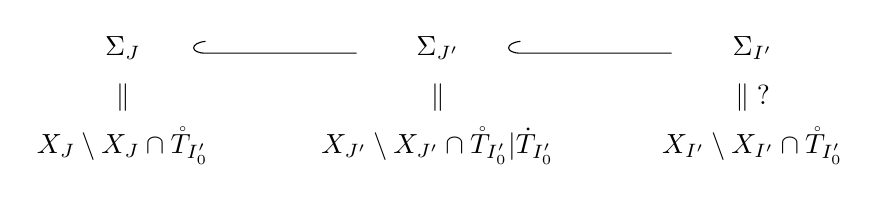
\begin{tikzpicture}[x=1cm,y=1cm]
\node at (0,0) {$\Sigma_J$};
\node at (4,0) {$\Sigma_{J'}$};
\node at (8,0) {$\Sigma_{I'}$};
\draw (1.05,0.09) .. controls (0.85,0.07) and (0.85,-0.06) .. (1.05,-0.06) -- (2.97,-0.06);
\draw (5.05,0.09) .. controls (4.85,0.07) and (4.85,-0.06) .. (5.05,-0.06) -- (6.97,-0.06);
\node at (0,-0.62) {$\Vert$};
\node at (4,-0.62) {$\Vert$};
\node at (8,-0.62) {$\Vert\;?$};
\node at (0,-1.24) {$X_J\setminus X_J\cap\mathring T_{I'_0}$};
\node at (4,-1.24) {$X_{J'}\setminus X_{J'}\cap\unsure{\mathring T_{I'_0}|\dot T_{I'_0}}$};
\node at (8,-1.24) {$X_{I'}\setminus X_{I'}\cap\mathring T_{I'_0}$};
\end{tikzpicture}}
Considérons donc le voisinage tubulaire de $\Sigma_J$ dans $\Sigma_{I'}$
\margin{85}
